\documentclass{bmvc2k}

% For the final submission, comment out the bmvcreviewcopy so that
% author names etc appear.
%\bmvcreviewcopy{1234}

\title{Author Guidelines for the\\ British Machine Vision Conference}

% Enter the paper's authors in order
% \addauthor{Name}{email/homepage}{INSTITUTION_CODE}
\addauthor{Susan Student}{http://www.vision.inst.ac.uk/~ss}{1}
\addauthor{Petra Prof}{http://www.vision.inst.ac.uk/~pp}{1}
\addauthor{Colin Collaborator}{colin@collaborators.com}{2}

% Enter the institutions
% \addinstitution{Name\\Address}
\addinstitution{
 The Vision Institute\\
 University of Borsetshire\\
 Wimbleham, UK
}
\addinstitution{
 Collaborators, Inc.\\
 123 Park Avenue,\\
 New York, USA
}

%Enter a shortened version of the title as a running header.
% For two authors, enter both surnames, separated by commas.  For
% more than two authors, the first author's name followed by
% \bmvaEtAl will produce the correct output (uppercase author name,
% lowercase etal).
\runninghead{Student, Prof, Collaborator}{BMVC Author Guidelines}

% Any macro definitions you would like to include
% These are not defined in the style file, because they don't begin
% with \bmva, so they might conflict with the user's own macros.
% The \bmvaOneDot macro adds a full stop unless there is one in the
% text already.
\def\eg{\emph{e.g}\bmvaOneDot}
\def\Eg{\emph{E.g}\bmvaOneDot}
\def\etal{\emph{et al}\bmvaOneDot}

%-------------------------------------------------------------------------
% Document starts here
\begin{document}

\maketitle

\begin{abstract}
This document demonstrates the format requirements for papers submitted
to the British Machine Vision Conference.  The format is designed for
easy on-screen reading, and to print well at one or two pages per sheet.
Additional features include: pop-up annotations for
citations~\cite{Authors06,Mermin89}; a margin ruler for reviewing; and a
greatly simplified way of entering multiple authors and institutions.

{\bf All authors are encouraged to read this document}, even if you have
written many papers before.  As well as a description of the format, the
document contains many instructions relating to formatting problems and
errors that are common even in the work of authors who {\em have}
written many papers before.
\end{abstract}

%-------------------------------------------------------------------------
\section{Introduction}
\label{sec:intro}
From 2009, the proceedings of BMVC (the British Machine Vision
Conference) will be published only in electronic form.  This document
illustrates the required paper format, and includes guidelines on
preparation of submissions.  Papers which fail to adhere to these
requirements may be rejected at any stage in the review process.

\LaTeX\ users should use this template in order to prepare their paper.
Users of other packages should emulate the style and layout of this
example.  Note that best results will be achieved using {\tt pdflatex},
which is available in most modern distributions.

\subsection{Paper length: nine pages plus bibliography and title}
Papers must be 9~pages in length, {\em excluding} the bibliography.  Length
is counted from the bottom of the title on the first page.  Therefore, the
bibliography should begin eight lines into page ten.  This is an
approximate measure, intended to encourage brevity, but authors should keep
in mind that blatant disregard of this instruction will cause reviewers to
require greater originality and impact of the submission.  {\bf Papers which are
clearly overlength will not be reviewed}.  This includes papers where the
margins and formatting are deemed to have been significantly altered from
those laid down by this style guide.  The reason such papers will not be
reviewed is that there is no provision for supervised revisions of
manuscripts.  The reviewing process cannot determine the suitability of the
paper for presentation in nine pages if it is reviewed in twelve.

The bibliography should begin immediately after the paper text.  It may
be of any length, within reason.  It should {\em not} include
annotations, figures, or any other paraphernalia intended to subvert the
paper length requirement.

\begin{figure}
\begin{tabular}{ccc}
\bmvaHangBox{\fbox{\parbox{2.7cm}{~\\[2.8mm]
\rule{0pt}{1ex}\hspace{2.24mm}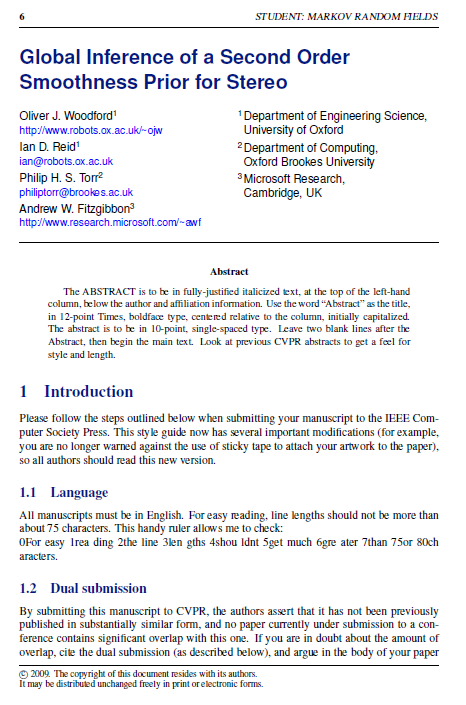
\includegraphics[width=2.33cm]{images/eg1_largeprint.png}\\[-0.1pt]}}}&
\bmvaHangBox{\fbox{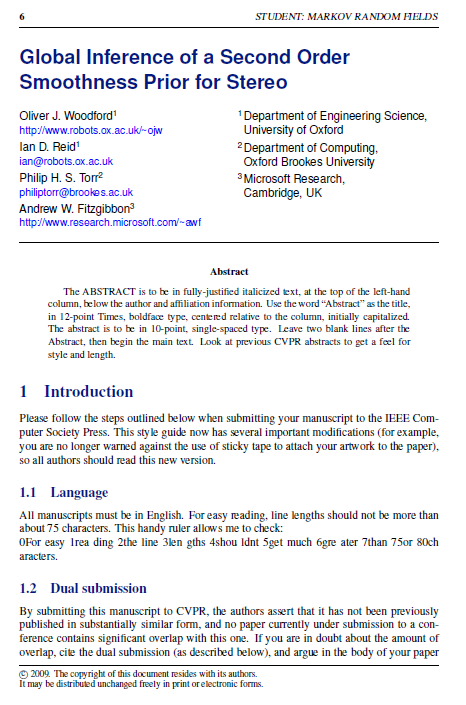
\includegraphics[width=2.8cm]{images/eg1_largeprint.png}}}&
\bmvaHangBox{\fbox{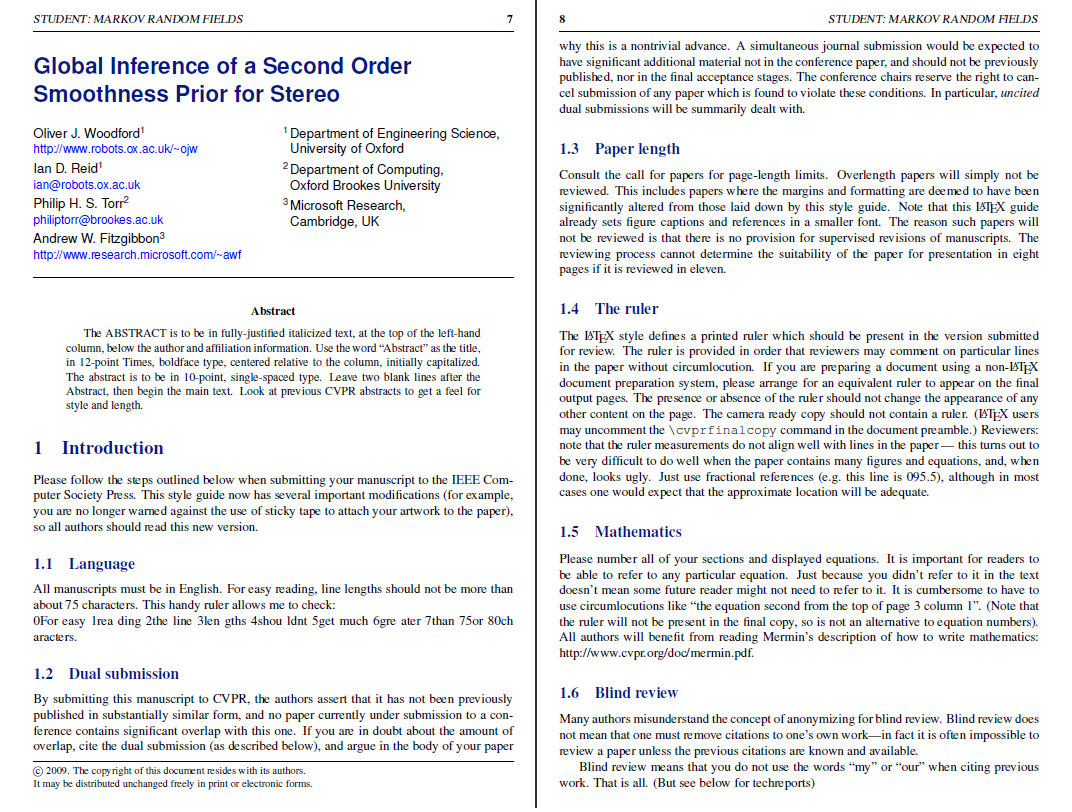
\includegraphics[width=5.6cm]{images/eg1_2up.png}}}\\
(a)&(b)&(c)
\end{tabular}
\caption{It is often a good idea for the first figure to attempt to
encapsulate the article, complementing the abstract.  This figure illustrates
the various print and on-screen layouts for which this paper format has
been optimized: (a) traditional BMVC print format; (b) on-screen
single-column format, or large-print paper; (c) full-screen two column, or
2-up printing. }
\label{fig:teaser}
\end{figure}

\subsection{Dual submission}
By submitting this manuscript to BMVC, the authors assert that it has not
been previously published in substantially similar form, and no paper
currently under submission to a conference contains significant overlap
with this one.  If you are in doubt about the amount of overlap, cite the
dual submission (as described below), and argue in the body of your paper
why this is a nontrivial advance.  A simultaneous journal submission would
be expected to have significant additional material not in the conference
paper, and should not be previously published, nor in the final acceptance
stages. The conference chairs reserve the right to cancel
submission of any paper which is found to violate these conditions.  In
particular, {\em uncited} dual submissions will be summarily dealt with.

\subsection{Anonymity and blind review}
BMVC operates a double-blind review process.  Your review submission {\bf
must not identify you as the author}.  This means, in particular, that the
author list should be replaced by the words ``BMVC {\em YYYY} Submission \#
{\em NNN}'', where the italics are to indicate the year and the submission
number.  The provided \LaTeX\ command \verb'\bmvcreviewcopy' does this
automatically.  In addition, acknowledgements should not be included in the
review copy.

Many authors misunderstand the concept of anonymizing for blind
review.  Blind review {\bf does not mean that one must remove
citations to one's own work}---in fact it is often impossible to
review a paper unless the previous citations are known and
available.

Blind review means that you do not use the words ``my'' or ``our''
when citing previous work.  That is all.  (But see below for
techreports)

Saying ``this builds on the work of Lucy Smith [1]'' does not say
that you are Lucy Smith, it says that you are building on her
work.  If you are Smith and Jones, do not say ``as we show in
[7]'', say ``as Smith and Jones show in [7]'' and at the end of the
paper, include reference 7 as you would any other cited work.

An example of a bad paper:
\begin{quote}
\begin{center}
    An analysis of the frobnicatable foo filter.
\end{center}

   In this paper we present a performance analysis of our
   previous paper [1], and show it to be inferior to all
   previously known methods.  Why the previous paper was
   accepted without this analysis is beyond me.

   [1] Removed for blind review
\end{quote}


An example of an excellent paper:

\begin{quote}
\begin{center}
     An analysis of the frobnicatable foo filter.
\end{center}

   In this paper we present a performance analysis of the
   paper of Smith \etal [1], and show it to be inferior to
   all previously known methods.  Why the previous paper
   was accepted without this analysis is beyond me.

   [1] Smith, L and Jones, C. ``The frobnicatable foo
   filter, a fundamental contribution to human knowledge''.
   Nature 381(12), 1-213.
\end{quote}

If you are making a submission to another conference at the same time,
which covers similar or overlapping material, you will almost certainly
need to refer to that submission in order to explain the differences,
just as you would if you or others had previously published related
work.  In such cases, include the anonymized parallel
submission~\cite{Authors06} as additional material and cite it as
\begin{quote}
[1] Authors. ``The frobnicatable foo filter'', ECCV 2006 Submission ID 324,
Supplied as additional material {\tt eccv06.pdf}.
\end{quote}

Finally, you may feel you need to tell the reader that more details can be
found elsewhere, and refer them to a technical report.  For conference
submissions, the paper must stand on its own, and not {\em require} the
reviewer to go to a techreport for further details.  Thus, you may say in
the body of the paper ``further details may be found
in~\cite{Authors06b}''.  Then submit the techreport as additional material.
Again, you may not assume the reviewers will read this material.

Sometimes your paper is about a problem which you tested using a tool which
is widely known to be restricted to a single institution.  For example,
let's say it's 1969, you have solved a key problem on the Apollo lander,
and you believe that the ICLL'70 audience would like to hear about your
solution.  The work is a development of your celebrated 1968 paper entitled
``Zero-g frobnication: How being the only people in the world with access to
the Apollo lander source code makes us a wow at parties'', by Zeus \etal.

You can handle this paper like any other.  Don't write ``We show how to
improve our previous work [Anonymous, 1968].  This time we tested the
algorithm on a lunar lander [name of lander removed for blind review]''.
That would be silly, and would immediately identify the authors. Instead
write the following:
\begin{quotation}
\noindent
   We describe a system for zero-g frobnication.  This
   system is new because it handles the following cases:
   A, B.  Previous systems [Zeus et al. 1968] didn't
   handle case B properly.  Ours handles it by including
   a foo term in the bar integral.

   ...

   The proposed system was integrated with the Apollo
   lunar lander, and went all the way to the moon, don't
   you know.  It displayed the following behaviours
   which show how well we solved cases A and B: ...
\end{quotation}
As you can see, the above text follows standard scientific convention,
reads better than the first version, and does not explicitly name you as
the authors.  A reviewer might think it likely that the new paper was
written by Zeus \etal, but cannot make any decision based on that guess.
He or she would have to be sure that no other authors could have been
contracted to solve problem B.

FAQ: Are acknowledgements OK?  No.  Leave them for the final copy.

\subsection{Citations}
When citing a multi-author paper, you may save space by using ``{\em et
alia}'', shortened to ``\etal'' (not ``{\em et.\ al.}'' as ``{\em et}'' is
a complete word.)  The provided \verb'\etal' macro is a useful {\em aide
memoire} in this regard.  However, use it only when there are three or more
authors.  Thus, the following is correct: `` Frobnication has been trendy
lately.  It was introduced by Alpher~\cite{Alpher02}, and subsequently
developed by Alpher and Fotheringham-Smythe~\cite{Alpher03}, and Alpher
\etal~\cite{Alpher04}.''

This is incorrect: ``... subsequently developed by Alpher \etal~\cite{Alpher03} ...''
because reference~\cite{Alpher03} has just two authors.  If you use the
\verb'\etal' macro, then you need not worry about double periods
when used at the end of a sentence as in Alpher \etal.

%For this citation style, keep multiple citations in numerical (not
%chronological) order, so prefer
We use {\tt natbib}, so citations in random order are nicely sorted:
 \cite{Alpher03,Alpher02,Authors06b,Authors06}.  However, we don't use the
compress option, as we want each reference to have its own hyperlink and
popup window.

%-------------------------------------------------------------------------
\subsection{Footnotes}

Please use footnotes\footnote {This is what a footnote looks like.  It
often distracts the reader from the main flow of the argument.} sparingly.
Indeed, try to avoid footnotes altogether and include necessary peripheral
observations in
the text (within parentheses, if you prefer, as in this sentence).  If you
wish to use a footnote, place it at the bottom of the column on the page on
which it is referenced. Use Times 8-point type, single-spaced.


\begin{figure*}
\begin{center}
\fbox{\rule{0pt}{2in} \rule{.9\linewidth}{0pt}}
\end{center}
   \caption{Example of a short caption, which should be centered.}
\label{fig:short}
\end{figure*}

%-------------------------------------------------------------------------
\subsection{The ruler}
The \LaTeX\ style defines a printed ruler which should be present in the
version submitted for review.  The ruler is provided in order that
reviewers may comment on particular lines in the paper without
circumlocution.  If you are preparing a document using a non-\LaTeX\
document preparation system, please arrange for an equivalent ruler to
appear on the final output pages.  The presence or absence of the ruler
should not change the appearance of any other content on the page.  The
camera ready copy should not contain a ruler. (\LaTeX\ users may remove
the \verb'[review]' option from the \verb'\documentclass' statement.)
Reviewers: note that the ruler measurements do not align well with lines
in the paper --- this turns out to be very difficult to do well when the
paper contains many figures and equations, and, when done, looks ugly.
Just use fractional references (e.g.\ this line is $210.5$), although in
most cases one would expect that the approximate location ($210$ in the
previous example) will be adequate.


\begin{table}
\begin{center}
\begin{tabular}{|l|c|}
\hline
Method & Frobnability \\
\hline\hline
Theirs & Frumpy \\
Yours & Frobbly \\
Ours & Makes one's heart Frob\\
\hline
\end{tabular}
\end{center}
\caption{Results.   Ours is better.}
\end{table}

\subsection{Mathematics}

Please number all of your sections and displayed equations.  It is
important for readers to be able to refer to any particular equation.  Just
because you didn't refer to it in the text doesn't mean some future reader
might not need to refer to it.  It is cumbersome to have to use
circumlocutions like ``the equation second from the top of page 3 column
1''.  (Note that the ruler will not be present in the final copy, so is not
an alternative to equation numbers).  All authors will benefit from reading
Mermin's description~\cite{Mermin89} of how to write mathematics.


%-------------------------------------------------------------------------
\subsection{References}

List and number all bibliographical references in 9-point Times,
single-spaced, at the end of your paper. When referenced in the text,
enclose the citation number in square brackets, for
example~\cite{Authors06}.  Where appropriate, include the name(s) of
editors of referenced books.


%------------------------------------------------------------------------
\subsection{Color}

Color is valuable, and will be visible to readers of the electronic copy.
However ensure that, when printed on a monochrome printer, no important
information is lost by the conversion to grayscale.

\bibliography{egbib}
\end{document}
